\subsection{ZFS I/O流水线}
\subsubsection{zfs\_write}
\begin{figure}[!h]
  \centering
  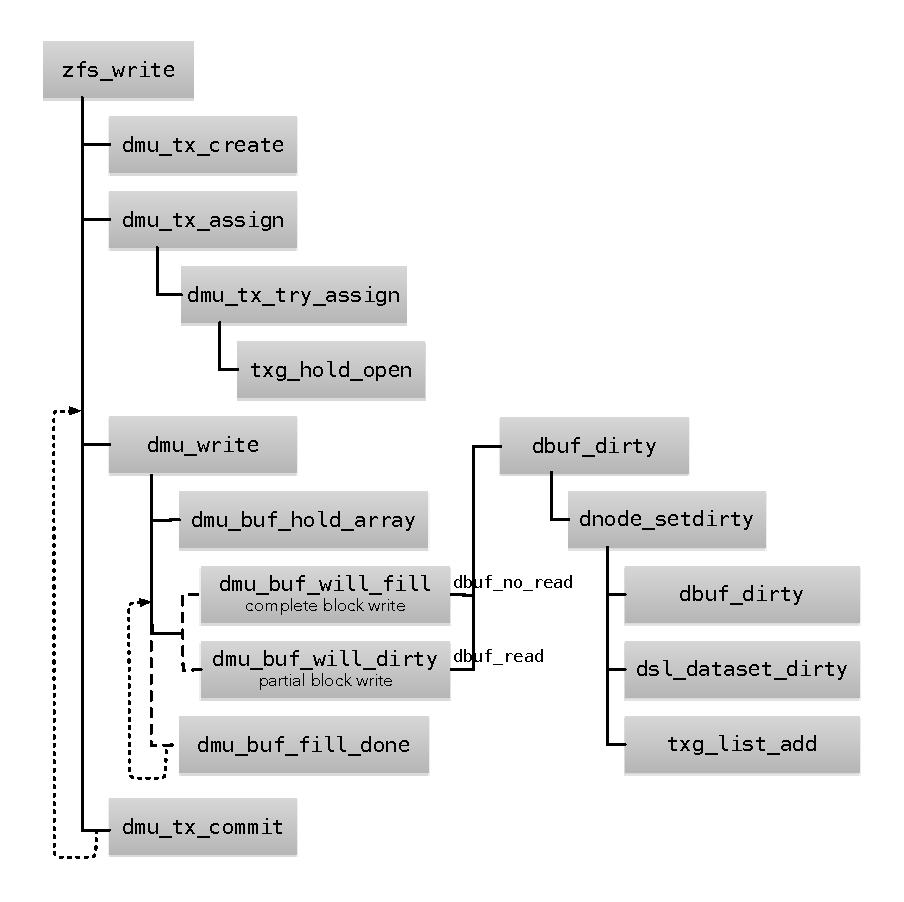
\includegraphics[scale=0.85]{fig/zfs_write.pdf}
  \caption{ZFS 写请求处理流程}\label{fig:zfs_write}
\end{figure}

系统调用和ZFS在写操作方面的交界点在\verb|zfs_write|函数,
此函数从用户空间获取数据并传给DMU层完成写入。
如果用户数据量大就需要将数据分成多个块,
为每一个块开启一个事务,
将事务加入事务组,
写数据块将触发一系列上游节点数据的更新,
将所有的更新都加入同一事务组。
大致调用链如图\,\ref{fig:zfs_write}\,所示。
最后一步提交事务,
负责处理事务组的线程被唤醒,
将事务取下,
完成对物理设备的写入工作。

\subsubsection{事务组}
一个事务组经历三个状态,
\begin{itemize}
  \item open: 新创建事务组即处于open状态,
    对内存中数据结构的更新在这状态中完成
  \item quiescing: 一个缓冲状态,
    这个状态的目的是等待所有组内的事务被提交,
    即过了此阶段,
    不会再有新的事务进入这个事务组,
    一般处于这个状态的事件都很短暂
  \item syncing: 在这个状态,
    将内存中更新写入永久存储介质
\end{itemize}

当创建或加载一个存储池时,
两个事务组线程被创建,
一个负责quiesce,
另一个负责sync。

负责sync的线程被唤醒之后调用\verb|spa_sync|函数,
从这个点到最后触发zio的调用链如图\,\ref{fig:spa_sync}\,所示。
\verb|dsl_pool_sync| 中 \verb|dsl_dataset_sync| 被调用了两次,
每一次都阻塞等带 I/O 返回,
在这一步 I/O 失败被认为是很严重事件,
kernel panic。

\begin{figure}[!ht]
  \centering
  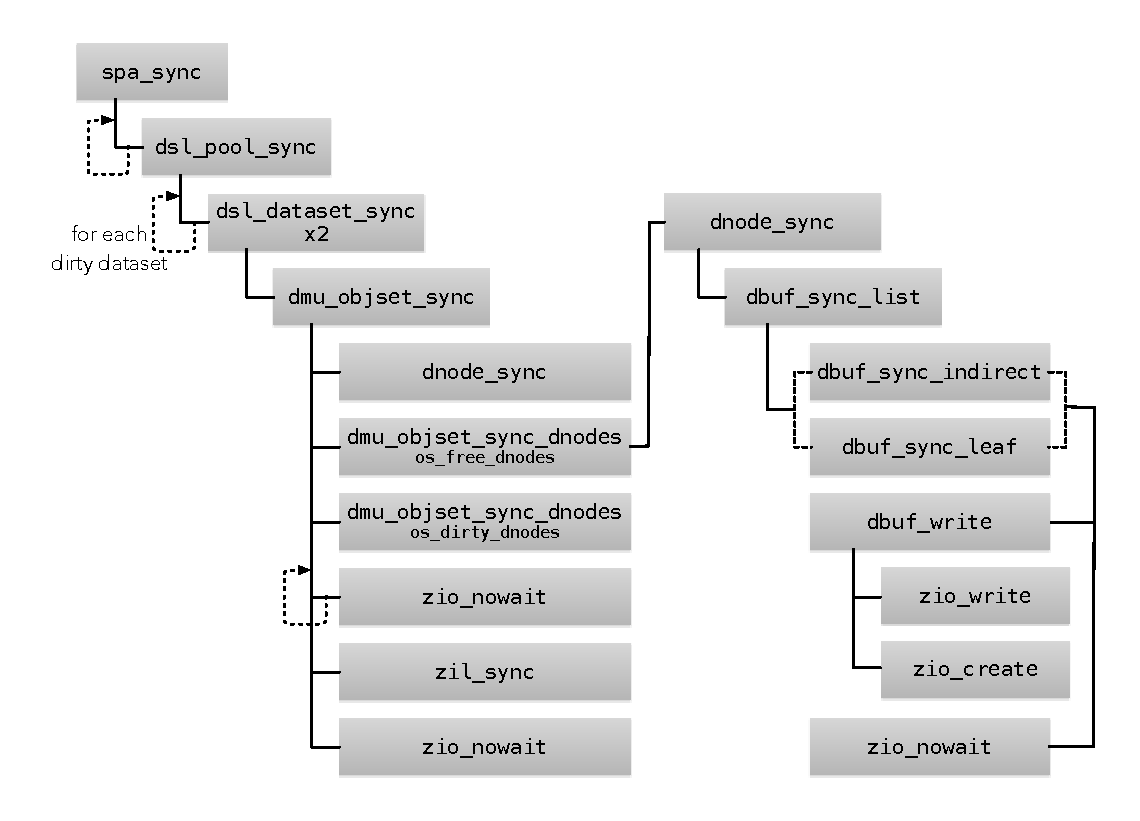
\includegraphics[width=\textwidth]{fig/zfs_spa_sync.pdf}
  \caption{sync到zio的流程}\label{fig:spa_sync}
\end{figure}

\verb|dbuf_sync_leaf|将数据异步地写出。
为了支持 COW,
数据块更新几次,
间接块必须相应更新几次。
\verb|dbuf_sync_indirect|函数对间接块进行读、修改其内容,
创建 ZIO 而后执行写出。

\subsubsection{I/O流水线}
执行 ZIO 的线程不是将整个I/O过程从头至尾执行,
为了提高吞吐率,
充分利用多核特性,
I/O被分为多道工序,
以优化方式分配给流水线上的工作线程。

I/O操作分为五类,
\begin{enumerate*}[label=\itshape\arabic*\upshape)]
  \item Read
  \item Write
  \item Free
  \item Claim
  \item Ioctl
\end{enumerate*}
这五类操作由不同的工序按指定顺序组合而成。

ZIO流水线的核心函数是\verb|zio_execute|。
和工厂流水线上工人一人只负责某几道确定工序不同,
ZIO 的线程可以负责任意工序,
一个线程完成某道工序之后有两种可能,
如果工序例程调用\verb|zio_taskq_dispatch|将
将半成品挂到某个队列上返回\verb|ZIO_PIPELINE_STOP|,
\verb|zio_execute|停止执行,返回,
之后工序交给谁处理由上一层逻辑按优化方式决定(当然可能还是同一个线程);%
\footnote{这里可能有优化余地,
  即让线程自己根据优化逻辑决定是挂出半成品还是自己继续处理}
否则例程会返回\verb|ZIO_PIPELINE_CONTINUE|,
当前线程在\verb|zio_execute|中继续调用下一道工序例程。

Write:
举例来说,
写操作的流水线定义如下:

\begin{lstlisting}{lanuage=C}
#define ZIO_WRITE_COMMON_STAGES		\
        (ZIO_INTERLOCK_STAGES	|	\
         ZIO_VDEV_IO_STAGES	|	\
         ZIO_STAGE_ISSUE_ASYNC	|	\
         ZIO_STAGE_CHECKSUM_GENERATE)
\end{lstlisting}

根据定义:

\begin{lstlisting}{lanuage=C}
 ZIO_STAGE_READY		= 1 << 16,	/* RWFCI */
 ZIO_STAGE_DONE			= 1 << 21,	/* RWFCI */
 ZIO_STAGE_VDEV_IO_START	= 1 << 17,	/* RWF-I */
 ZIO_STAGE_VDEV_IO_DONE		= 1 << 18,	/* RWF-- */
 ZIO_STAGE_VDEV_IO_ASSESS	= 1 << 19,	/* RWF-I */
 ZIO_STAGE_ISSUE_ASYNC		= 1 << 3,	/* RWF-- */
 ZIO_STAGE_CHECKSUM_GENERATE	= 1 << 5,	/* -W--- */
\end{lstlisting}

各道工序的例程在\verb|zio_pipeline|中定义:
\begin{lstlisting}{language=C}
static zio_pipe_stage_t *zio_pipeline[] = {
	NULL,
	zio_read_bp_init,
	zio_free_bp_init,
	zio_issue_async,
	zio_write_bp_init,
	zio_checksum_generate,
	zio_nop_write,
	zio_ddt_read_start,
	zio_ddt_read_done,
	zio_ddt_write,
	zio_ddt_free,
	zio_gang_assemble,
	zio_gang_issue,
	zio_dva_allocate,
	zio_dva_free,
	zio_dva_claim,
	zio_ready,
	zio_vdev_io_start,
	zio_vdev_io_done,
	zio_vdev_io_assess,
	zio_checksum_verify,
	zio_done
};
\end{lstlisting}

也就是说要完成\verb|zio_write|,
以下流水线上函数将被依次调用:
\begin{lstlisting}{lanuage=C}
 zio_issue_async,
 zio_checksum_generate,
 zio_ready,
 zio_vdev_io_start,
 zio_vdev_io_done,
 zio_vdev_io_assess,
 zio_done
\end{lstlisting}

\verb|zio_issue_async|函数将zio挂如一个taskq线程的队列,
告知\verb|zio_execute|立即返回,
taskq线程完成余下工作。

\verb|zio_checksum_generate|函数生成较验和之后返回
\verb|ZIO_PIPELINE_CONTINUE|,
于是该taskq线程继续下一道工序,即\verb|zio_ready|。

\verb|zio_ready|一开始调用\verb|zio_wait_for_children|,
如果zio有gang或者ddt类型的子zio,
\verb|zio_wait_for_children|将工序移至下一道,
但状态设为{\em stall}并返回stop,
使得\verb|zio_execute|直接返回,
zio的工序暂停,
直至所有子zio都到达\verb|READY|阶段以后才能继续执行。
\verb|zio_ready|将调用\verb|zio_notify_parent|,
\verb|zio_notify_parent|又调用\verb|zio_execute|%
继续父zio刚才暂停的工序,
当然并非一定是该线程完成,
依然可能是将zio挂到某个taskq的队列中就返回。

下一道工序是\verb|zio_vdev_io_start|,
它负责为物理I/O做准备。
如果该zio的vdev是物理设备,
调用\verb|vdev_queue_io|将zio挂入vdev的队列,
返回\verb|STOP|;
否则直接调用该设备的\verb|vdev_op_io_start|%
(可能是mirro,或者Raid等等)
方法将zio逐层下传至物理设备。
这一道工序总是返回\verb|STOP|。

\verb|zio_vdev_op_io_done|主要就是错误处理,
之后就是收尾的两道工序。

\subsubsection{ARC及L2ARC}
LRU:
考虑如下场景,
当程序一次性地读入大量数据(常见的例如:\verb|grep -nr|),
那些数据块轻易填满cache,
挤出大量的页,
但它们仅仅被使用一次,
滞留在cache中毫无益处。
那些被频繁使用的页却被无谓地换出。
另外一方面,
单单考虑页面访问频度的策略也有其缺陷,
ARC的思路是同时采纳两种策略,
并且自适应地在二者间做权衡。

ARC:
ARC维护两个先进先出的页面队列,
分别存放按MRU和MFU策略处理的页描述子。
MRU和MFU还各自有一个ghost队列。
页面第一次被读入并缓存时,
插入MRU队列头部,
当它第二次被访问就移入MFU队列,
在MFU队列中再次被访问则会移到队列头。
当cache够用时,
两个ghost队列都为空,
MFU和MRU各自扩张到最大限度。
如图\,\ref{fig:zfs_arc0}\,所示。

\begin{figure}[!h]
  \centering
  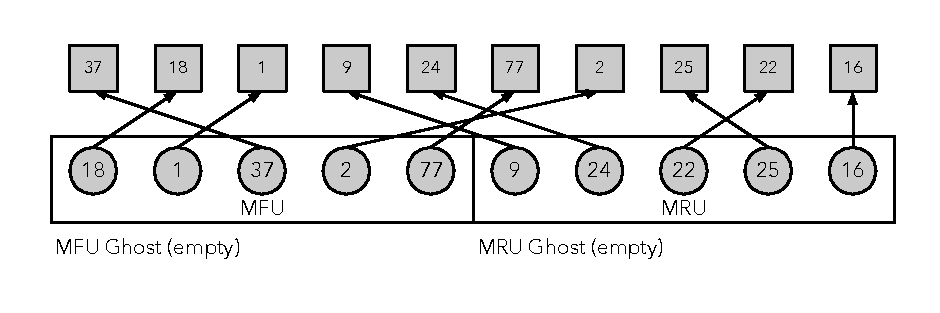
\includegraphics[width=\textwidth]{fig/zfs_arc0.pdf}
  \caption{MSU和MRU}\label{fig:zfs_arc0}
\end{figure}

\begin{figure}[!ht]
  \centering
  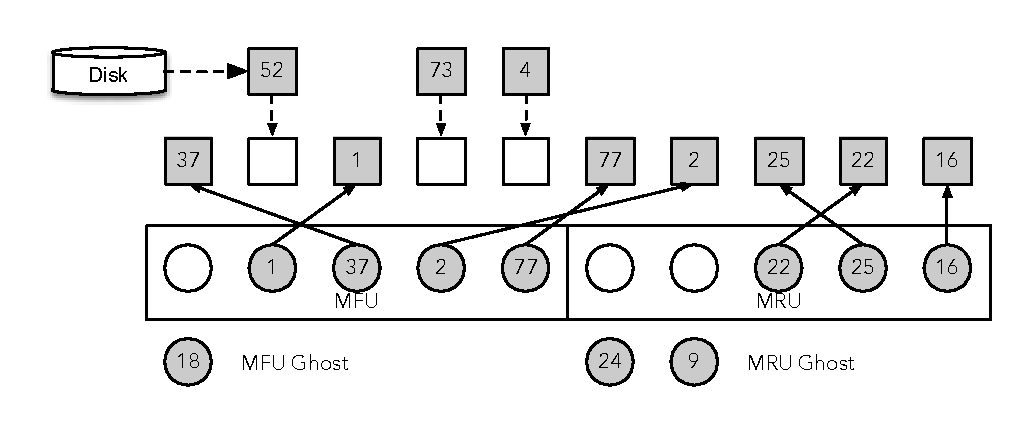
\includegraphics[width=\textwidth]{fig/zfs_arc1.pdf}
  \caption{Evicted to Ghost Lists}\label{fig:zfs_arc1}
\end{figure}

内存紧张以后,
再从磁盘读入新页将触发cache中某些页面被清除({\em evict}),
这时将该页面的描述子插入其所属页缓存类的ghost队列头,
即虽然磁盘数据块已经不在内存中,
其引用依然保留。
当然ghost队列越来越长到达最大限度以后,
页面的描述子将被依次序删除,
对应磁盘数据块的引用彻底消失。
图\,\ref{fig:zfs_arc1}\,演示了页面被evict的场景。

当已换出数据块再次被从磁盘读取,
如果发现其引用仍位于某个的ghost队列中,
这透露的一个信息是该类页缓存的miss率较高,
需要增加该类页缓存的额度,
当然同时减少另外一方的额度,
图\,\ref{fig:zfs_arc2}\,演示了这一过程。

\begin{figure}[!ht]
  \centering
  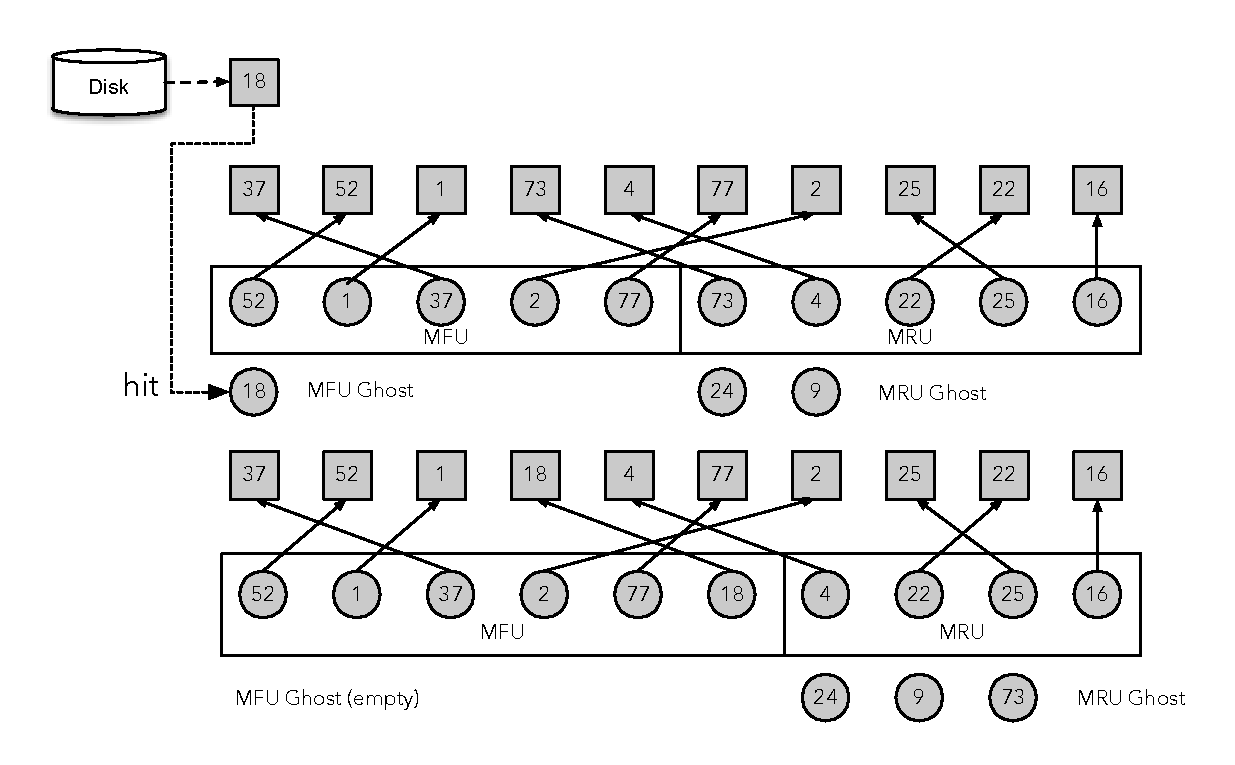
\includegraphics[width=\textwidth]{fig/zfs_arc2.pdf}
  \caption{Expand MFU and Shrink MRU}\label{fig:zfs_arc2}
\end{figure} 

两类页缓存策略采用相同的逻辑,
两种策略自适应地趋向符合work load的页使用需求。
仍然考虑之前的场景,
一次性读入大量数据导致MRU的ghost队列很长,
但它们再没有被命中过,
如果有其它的应用%
\footnote{譬如数据库在某些时候会反复执行相同的查询}%
使得MFU的ghost队列总是命中,
于是MFU的页缓存队列越来越长而MRU的页缓存队列越来越短,
逐渐达到平衡,
页面的换出策略得到优化。

ZFS对ARC的实现与源算法有些小区别。
\begin{itemize}
  \item ZFS 的缓存容量根据当前可用内存动态可变;
  \item ZFS 支持多种不同块尺寸;
  \item ZFS 支持把一个页锁在内存种,
    在清除页时需要扫一下队列找最老的可清除的页。
\end{itemize}

L2ARC:
可以让ZFS使用SSD作为二级页缓存设备,
即所谓{\em L2ARC},
它使用了一个\verb|l2arc_only|队列维护只在SSD上的页缓存。
其主要算法和ARC完全一致。
一个自然的想法使当ARC需要清除页面时,
自动地清到SSD上。
但这样将导致一些严重问题,
其一是当有一个大数据读将一次刷出大量页面到SSD上,
其二是当应用程序开辟大量内存是,
ARC需要被缩减,这时又可能导致一次性大量页面刷出。
ZFS解决方法是用一个线程\verb|l2arc_feed_thread|扫描两个缓存队列,
将最近可能要清除出去的页组到一个8M的缓冲区,
之后由另一个\verb|write_hand|线程一次性写出,
这适当降低了突发大量写的危害。
